\begin{figure}[t]
\centering
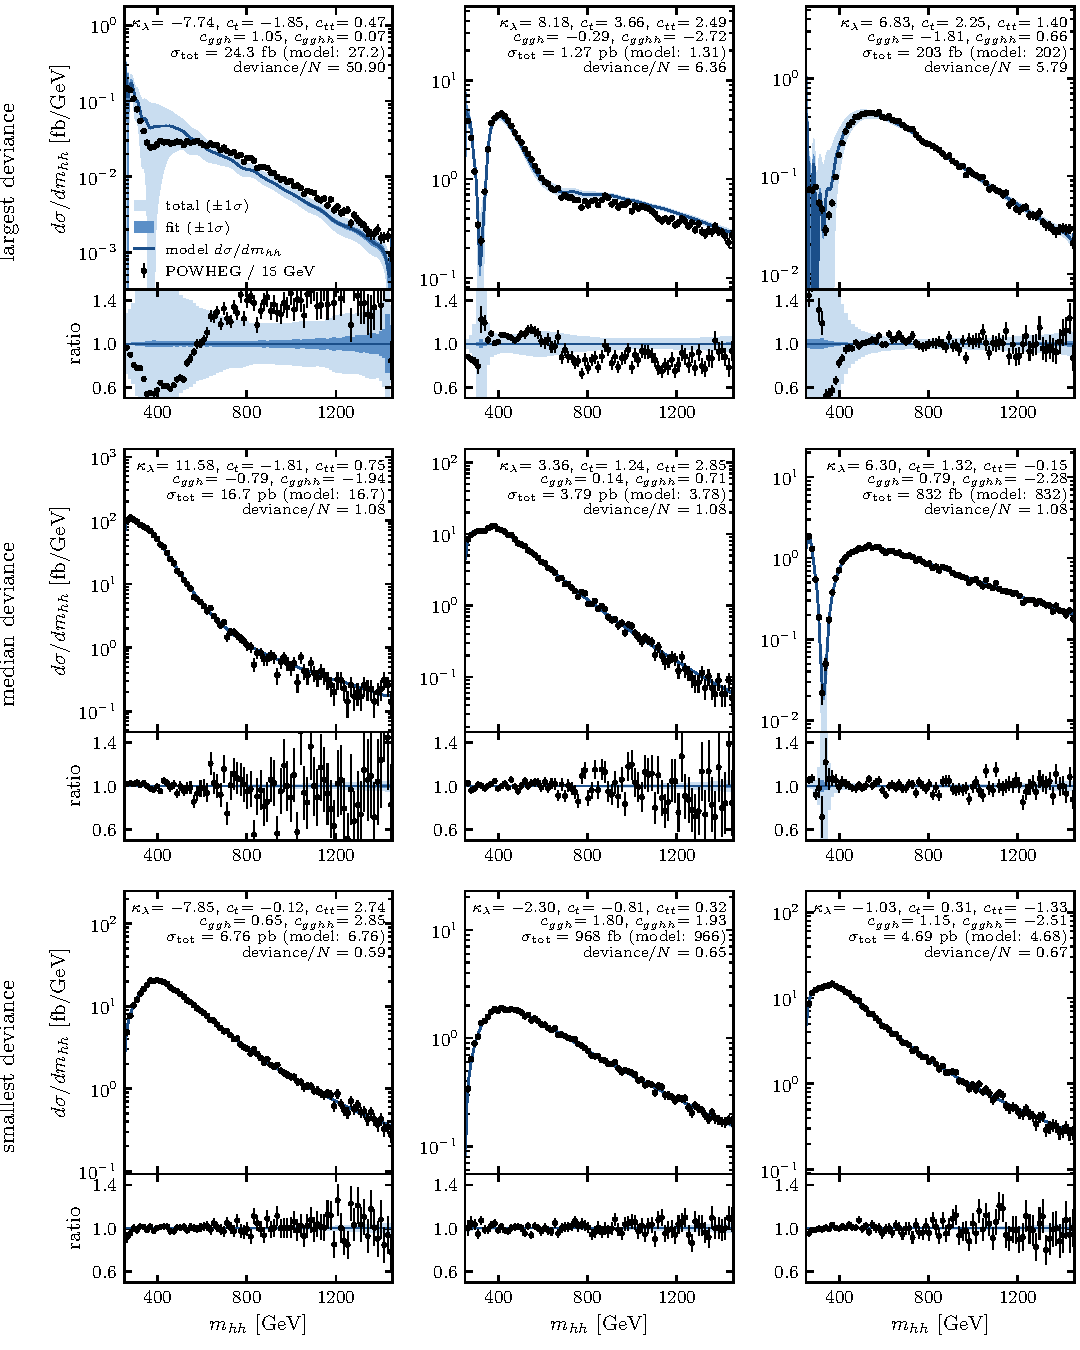
\includegraphics[width=\textwidth]{fig_spectra_panel.pdf}
\caption{POWHEG spectra divided by the bin width (points; error bars: Poisson noise) and the smooth
model's density $d\sigma/dm_{hh}$ (line) for nine of the 1,000 test spectra, ranked by the Poisson
deviance per bin: the three largest (top), three around the median (middle) and the three smallest
(bottom). Dark band: fit uncertainty ($\pm1\sigma$); light band: total, including the model
discrepancy. The lower panels show the ratio of POWHEG to the model's bin integrals. Each panel gives
the HEFT parameters, the total cross section in 255--1455~GeV from POWHEG and from the model, and the
deviance per bin. The largest deviances occur where the total cross section is smallest, through
destructive interference.}
\label{fig:spectra}
\end{figure}
